\chapter{A Credibilidade na Classificação Automática} 
\label{cap::metodo}

Como mostrado na Seção~\ref{cap::related}, o termo credibilidade já foi utilizado com diferentes significados na literatura. Nesse trabalho, iremos nos ater ao conceito de credibilidade no contexto de classificação automática. Assumimos que a credibilidade de uma entidade reflete o quanto de qualidade ela agrega em uma tarefa a ser executada. Sendo assim, para a tarefa de classificação, a credibilidade de uma entidade é diretamente proporcional ao tanto que aquela entidade ajuda na discriminação de uma classe. Isso significa que um documento $D_{1}$ tem um valor de credibilidade maior que outro documento $D_{2}$, caso ele forneça maiores indícios para descobrirmos a qual classe um terceiro documento $D_{3}$ pertence. Logo, definimos a credibilidade de uma entidade como um número real que incorpora diversos fatores quantitativamente em um único valor dentro de uma faixa predefinida, chamada de escala de credibilidade. Temos também que quanto maior é esse valor, mais importante essa entidade é para ajudar na tarefa de classificação. No contexto de classificação de textos, alguns fatores que podemos considerar são os termos, os autores, as citações, os meios de vinculação ou mesmo o ano de lançamento de um documento. O valor da credibilidade apresenta um comportamento assintótico crescente e monotônico, ou seja, ao calcularmos a credibilidade de uma entidade levando em conta todos os possíveis fatores produziremos um valor mais significativo de credibilidade do que quando calculamos levando em conta apenas um subconjunto desses fatores.

Já existem algumas métricas que podem ser usadas como ``funções de credibilidade'', como a distância média utilizada no algoritmo dos $K$ vizinhos mais próximos, \textit{KNN}. Nela quanto maior é a distância, menor é a credibilidade da informação provida. Podemos ainda definir algumas métricas que levam em consideração o valor discriminativo dos atributos de uma entidade, por exemplo as métricas \textit{TD-IDF} e \textit{dominância}. Ambas serão explicadas com maiores detalhes a seguir, na Seção~\ref{sec::pg_cred_baseada_conteudo}, entretanto, por enquanto, podemos dizer que a primeira provê um medida global de significância para um atributo, enquanto, a segunda provê um valor local. Uma boa ideia seria unir os benefícios providos por ambas, porém como realizar essa junção é um desafio. Uma abordagem simples é realizar uma soma de pesos provenientes de cada uma das métricas, porém essa pode ser uma abordagem muito simplista que não considera nenhuma correlação entre as métricas.

%versao com NB + KNN
Finalmente, uma vez definido um valor para a credibilidade, temos que utilizá-lo. Isso quer dizer que, no contexto de classificação automática, os algoritmos devem ser alterados de forma a levar em consideração o valor da credibilidade dos exemplos utilizados. Nesse trabalho, incorporamos a credibilidade em dois algoritmos clássicos, o \textit{Naïve Bayes} e o algoritmo dos $K$ vizinhos mais próximos, \textit{KNN}. O principal motivo para utilizarmos o \textit{Naïve Bayes} é que esse apresenta um bom desempenho, especificamente para classificação de documentos (\cite{salles10}), que é o principal tipo de classificação que tratamos nesse trabalho. Embora o algoritmo \textit{Support Vector Machine}, \textit{SVM}, possa superar o \textit{Naïve Bayes} em alguns cenários de classificação de documentos, o custo computacional de utilizar o \textit{SVM} em um problema de classificação multi-rótulo é um problema a ser levado em conta. Baseado no compromisso entre o custo computacional e os resultados obtidos, decidimos por utilizarmos o algoritmo \textit{Naïve Bayes}, detalhado na Seção~\ref{subsec::cred_nb}. Entretanto, gostaríamos de mostrar que a credibilidade não está presa a apenas um classificador e, portanto, também realizamos modificações no \textit{KNN}. Escolhemos o \textit{KNN}, explicado na Seção~\ref{subsec::cred_knn}, por sua simplicidade, apresentando apenas um parâmetro, seus bons resultados em bases de bio-informática (citar) e por advogarmos que o \textit{KNN} já utiliza uma credibilidade básica em sua própria estrutura. Finalmente, as Seções~\ref{subsubsec::nb_cred} e \ref{subsubsec::knn_cred} abordam como podemos incorporar as funções de credibilidade nos algoritmos \textit{Naïve Bayes} e \textit{KNN}, respectivamente.

%Versao onde so temos o NB:
% Finalmente, uma vez definido um valor para a credibilidade de uma entidade, temos que utilizá-lo. Isso quer dizer que, no contexto de classificação automática, os algoritmos devem ser alterados de forma a levar em consideração o valor da credibilidade dos exemplos utilizados. Nesse trabalho, focamos no algoritmo \textit{Naïve Bayes} (mudar depois?!), pois esse apresenta um bom desempenho, especificamente para classifição de documentos~\cite{salles10}, que é o principal tipo de classificação que tratamos nesse trabalho. Embora o algoritmo SVM possa superar o \textit{Naïve Bayes} em alguns cenários de classificação de documentos, o custo computational de utilizar o SVM em um problema de classificação multi-rótulo é um problema a ser levado em conta. Baseado no compromisso entre o custo computacional e os resultados obtidos, decidimos por utilizarmos o algoritmo \textit{Naïve Bayes}, detalhado na Seção ~\ref{sec::cred_classificadores}.

%%%%%%%%%%%%%%%%%%%%------------------------------------------------------------------------------------------------------------------------------------%%%%%%%%%%%%%%%%%%%%%%%%%%%%%%%%%
%%%%%%%%%%%%%%%%%%%%------------------------------------------------------------------------------------------------------------------------------------%%%%%%%%%%%%%%%%%%%%%%%%%%%%%%%%%
%%%%%%%%%%%%%%%%%%%%------------------------------------------------------------------------------------------------------------------------------------%%%%%%%%%%%%%%%%%%%%%%%%%%%%%%%%%

\section{Classificador \textit{Naïve Bayes}.}
\label{subsec::cred_nb}

%Nessa seção, incorporamos a credibilidade no classificador bayesiano. Primeiramente, definimos o funcionamento do algoritmo \textit{Naïve Bayes} original na Seção~\ref{subsubsec::nb_original} e posteriormente, discutimos como incorporamos o conceito de credibilidade no mesmo, na Seção~\ref{subsubsec::nb_cred}.

%\subsubsection{\textit{Naïve Bayes} original.}
%\label{subsubsec::nb_original}

Nessa seção, explicamos o funcionamento da versão original do algoritmo \textit{Naïve Bayes}. É importante termos em mente a versão original do mesmo para que possamos compará-lo com a versão na qual a credibilidade está inclusa, ver Seção~\ref{subsubsec::nb_cred}. Referências mais detalhadas podem ser encontradas em \cite{DHS01} e \cite{Manning08}.

De uma maneira sucinta, porém prática, podemos utilizar os seguintes passos para definir o classificador \textit{Naïve Bayes}:

\begin{enumerate}
    \item Cada um dos exemplos \footnote{Os nomes ``exemplo'' e ``instância'' são utilizados com o mesmo significado durante o todo o texto.} também chamados de instâncias, do conjunto de treinamento pode ser visto como um vetor (ou uma tupla) $D$-dimensional, $X$ = ($x_1$, $x_2$, $x_3$, ..., $x_d$), onde $x_i$ é o valor referente ao atributo $A_i$ no exemplo $X$. É importante ressaltar que para um atributo $A_i$, poderíamos ter valores distintos de $x_i$ nos vários exemplos de treino. Tipicamente, em um problema de classificação com atributos numéricos, o atributo $x_i$ pode assumir qualquer valor real. Já em um problema de classificação categórico, $x_i$ pode assumir uma faixa controlada de valores discretos. Em classificação de texto, por exemplo, $x_i$ pode ser qualquer valor inteiro natural, representando o número de vezes que temos um termo $A_i$ em $X$. Vale a pena lembrar também que podemos ter a coexistência de atributos numéricos e categóricos em uma mesma base de dados.
    

    \item Suponha que existem \textit{m} classes, $c_1$, $c_2$, ..., $c_\textit{m}$, formando o conjunto de possíveis classes $\mathbb{C}$. Dada uma determinada tupla $X$, o classificador Bayesiano irá predizer que $X$ pertence à classe que tiver a maior probabilidade a \textit{posteriori} $P(c_i|X)$, referente ao exemplo $X$. Ou seja, o classificador \textit{Naïve Bayes} dirá que a tupla $X$ pertence a $c_i$, se e somente se:
        
\begin{equation}\label{eqn::max_pcgivenx}
   P(c_{i}|X) > P(c_{j}|X) \;\;\;\;\;\forall j,\; 1 \le j \le m, \; j \not= i
\end{equation}

Onde, $P(A|B)$, como suposto, é um valor real entre 0.0 e 1.0 que define a probabilidade do evento A ser verdadeiro, dado que o evento B ocorreu. No caso, podemos interpretar a expressão $P(c_i|X)$ como a probabilidade da classe correta ser $c_i$ dado o exemplo $D$-dimensional $X$ = ($x_1$, $x_2$, ..., $x_d$).

    \item Necessitamos, portanto, uma forma de calcular a probabilidade a \textit{posteriori} $P(c_i| X)$, que pode ser definida pelo teorema de Bayes como:
 
\begin{equation}\label{eqn::bayes}
   P(c_{i}|X) = \frac{P(X|c_i) \times P(c_i) }{P(X)}
\end{equation}

    \item Da Equação~\ref{eqn::bayes} temos que $P(c_i)$ pode ser obtida simplesmente calculando a proporção de exemplos da classe $c_i$ que temos em nosso conjunto de treinamento. Além disso, como $P(X)$ é uma constante independente da classe, não precisamos de calcular esse fator.
       
    \item Calcular $P(X|c_i)$ é uma tarefa extremamente cara computacionalmente. Porém podemos utilizar a premissa ``ingênua'' \footnote{O nome do algoritmo Naïve Bayes provém dessa premissa simplificadora.} de que os valores dos atributos de um exemplo $X$ são condicionalmente independentes um dos outros, dada uma certa classe. Logo,

\begin{equation}\label{eqn::classindependence}
   P(X|c_{i}) = \prod^{n}_{k=1}{P(x_k|c_i) }
\end{equation}

\item O valor de cada termo $P(x_k|c_i)$ da Equação~\ref{eqn::classindependence} é usualmente calculado de forma diferente caso o atributo $A_i$ seja categórico ou numérico. A seguir mostramos as formas mais comuns vistas na literatura:
    \begin{itemize}

        \item Caso $A_k$ seja categórico, então $P(x_k|c_i)$ é o número de exemplos no treinamento que pertencem a classe $c_i$, nos quais o valor de $A_k$ é $x_k$, dividido pelo número de exemplos da classe $c_i$ no treino. De maneira especial, para o problema de classificação de documentos, podemos utilizar a mesma definição expressa na seguinte fórmula:

    \begin{equation}\label{eqn::nbcattexto}
        P(x_k|c_i) = \frac{ N_{x_{k}c_{i}} }{ \sum\limits^{d}_{1} { } N_{x_{l}c_{i}} } 
    \end{equation}

        Onde $N_{x_{k}c_{i}}$ é o número de vezes que temos o termo $x_k$ nos exemplos (aqui, documentos) da classe $c_i$ e $d$ é o número de atributos existentes (tamanho do vocabulário conhecido).

        \item Caso $A_k$ seja um atributo numérico, tipicamente um valor real, então assumimos que o valor $x_k$ do atributo $A_k$ é dado por uma distribuição Gaussiana de média $\mu_k$ e desvio padrão $\sigma_k$ e podemos usar a seguinte fórmula para calcular $P(x_k|c_i)$:
    \begin{eqnarray}\label{eqn::nbnumerico}
        P(x_k|c_i) & = & g(x_k, \mu_{kc_i}, \sigma_{kc_i})  \\
        g(x, \mu, \sigma) & = & \frac {1} { \sqrt{2\pi\sigma} } e^{ -\frac{(x-\mu)^2}{2\sigma^2}  } 
    \end{eqnarray}
        
        Onde $\mu_{kc_i}$ e $\sigma_{kc_i}$ são a média e o desvio padrão dos valores de $A_k$ nas tuplas de treinamento da classe $c_i$. 

    \end{itemize}

    \item Finalmente, podemos juntar as Equações \ref{eqn::max_pcgivenx} e \ref{eqn::classindependence}, definindo:

    \begin{equation}\label{eqn::nbfinal}
    \textit{Classe Atribuída} = \arg\max_{c_i \in M}P(X|c_i) = \frac{N_{c_i}}{N} \cdot {\prod^{n}_{k=1}{P(x_k|c_i) }}.
    \end{equation}

    Onde $N$ é o número de exemplos no conjunto de treinamento e $N_{c_i}$ é o número de exemplos da classe $c_i$ em $N$.


\end{enumerate}

%%%%%%%%%%%%%%%%%%%%------------------------------------------------------------------------------------------------------------------------------------%%%%%%%%%%%%%%%%%%%%%%%%%%%%%%%%%

\section{Incorporando a credibilidade no \textit{Naïve Bayes}.}
\label{subsubsec::nb_cred}

Nessa seção, explicamos como incorporar o conceito de credibilidade no classificador Bayesiano. Primeiramente, modelamos a credibilidade de um exemplo inspirado unicamente em seu conteúdo, assim como mostrado na Seção \ref{subsubsec::nbcredconteudo}. Por sua vez, na Seção \ref{subsubsec::nbcredgrafos}, mostramos como tratar a credibilidade em um nível mais alto, tentando tirar proveito das relações existentes entre as instâncias de treinamento e a instância de teste, a princípio, sem nos preocuparmos com seus conteúdos.

\subsection{\textit{Naïve Bayes} com credibilidade baseada no conteúdo.}
\label{subsubsec::nbcredconteudo}

A credibilidade de uma instância $X$, baseada no seu próprio conteúdo, procura determinar para cada atributo $A_k = x_k$ em $X$, o quanto $x_k$ contribui para conseguirmos predizer a qual classe $X$ pertence. De maneira geral, calculamos a credibilidade de $x_k$, referente ao atributo $A_k$ em relação a classe $c_i$, como uma função $Cr_{cont}(x_k, c_i)$ e podemos facilmente acoplá-la a Equação~\ref{eqn::classindependence}, resultando em:

\begin{equation}\label{eqn::classindependence_conteudo}
   P(X|c_{i}) = \prod^{D}_{k=1}{(P(x_k|c_i) \cdot Cr_{cont}(x_k,c_i))} 
\end{equation}

Dessa forma, avaliamos para cada atributo $A_k$ o quanto ganhamos sabendo que $A_k$ tem o valor de $x_k$, dada cada uma das classes $c_i$. Existem várias métricas conhecidas na literatura que podem ser utilizadas para medirmos a influência de um termo na determinação da classe de uma instância de teste, como o \textit{Ganho de informação} (IG - do inglês \textit{Information Gain}) e a \textit{Medida de Ambiguidade} (AM - do inglês \textit{Ambiguity Measure}), por exemplo. Ambas, como veremos, poderiam vir a ser boas funções de credibilidade. 


    Com um pouco mais de detalhe, a \textit{Medida da Ambiguidade} definida em \cite{Mengle08} procura verificar a importância do valor de atributo baseado no número de vezes que aquele valor aparece conjuntamente com uma determinada classe. Matematicamente, temos:
\begin{equation}\label{eqn::classindependence_conteudo_am}
   Cr_{cont} = AM(t_k, c_i) = \frac{ N_{t_{k}c_{i}}}{\sum_{c_j \in \mathbb{C}} N_{t_{k}c_{j}}}.
\end{equation}
   Onde $N_{t_{k}c_{j}}$ é o número de instâncias no treino onde $A_k$ vale $t_k$ e pertence a classe $c_j$. Especificamente, no problema de classificação de textos, $N_{t_{k}c_{j}}$ é a frequência do termo $t_k$ nos documentos de classe $c_j$.

    Por sua vez, o \textit{Ganho de Informação} (ver \cite{forman03}) mede o quanto de informação adquirimos para predizermos uma classe, sabendo o valor de um certo atributo. Estatisticamente, teríamos:
\begin{equation}\label{eqn::classindependence_conteudo_ig}
   Cr_{cont} = IG(t_k, c_i) = \sum_{c \in \{c_i, \overline{c_i}\}}\sum_{t \in \{t_k, \overline{t_k}\}}P(t|c)\log_2\frac{P(t|c)}{P(t)P(c)}.
\end{equation}

    Porém não sabemos qual das duas métricas funcionaria melhor como uma função de credibilidade, pois isso é uma tarefa dependente da aplicação. Além disso, poderíamos combinar essas métricas para conseguirmos uma função que venha a obter ainda melhores resultados. Na verdade, existem muitas outras métricas que podemos utilizar como função de credibilidade baseada no conteúdo. Listamos e explicamos cada uma das métricas que foram utilizadas nesse trabalho na Seção~\ref{subsec::pg_metricas_conteudo}. É importantíssimo destacar que devido ao grande número de métricas, testar uma a uma e as suas possíveis combinações é uma tarefa combinatória muito cara computacionalmente, e, portanto inviável. Por esse motivo, empregamos a \textit{Programação Genética} (PG), um mecanismo capaz de combinar essas métricas de forma elegante, formando funções de credibilidade mais robustas. (melhorar depois?!?!) Dedicamos o Capítulo~\ref{cap::programacao_genetica} exclusivamente para abordamos em detalhes como usamos PG na geração de funções.

%%%%%%%%%%%%%%%%%%%%------------------------------------------------------------------------------------------------------------------------------------%%%%%%%%%%%%%%%%%%%%%%%%%%%%%%%%%

\subsection{\textit{Naïve Bayes} com credibilidade baseada em relacionamentos.}
\label{subsubsec::nbcredgrafos}

A credibilidade da pertinência de um exemplo em uma classe também pode ser mensurada baseando nos relacionamentos existentes entre o exemplo e o conjunto de treinamento. Anteriormente, calculamos o quanto saber que um atributo $A_i$ tem valor $x_i$ nos ajuda a classificar um exemplo em relação a uma classe $c_j$. Dessa vez, gostaríamos de calcular o quanto ganhamos explorando os relacionamentos existentes entre nossa instância de teste e as instâncias de treinamento. Para tanto, necessitamos que um relacionamento possa ser estabelecido entre as entidades de nossa base de treinamento e teste. Alguns relacionamentos comuns na tarefa de classificação de texto, por exemplo, são autoria e citação. No primeiro, criamos um elo entre dois documentos se eles têm um mesmo autor em comum e, no segundo, criamos um elo entre eles se um cita ou é citado pelo outro. Teríamos relacionamentos bastante parecidos em uma base de músicas ou uma outra de vídeos. É oportuno destacar que podemos tratar todos esses relacionamentos como um grafo.

Formalmente, um grafo $G = (V,E)$ é uma estrutura composta por um conjunto $V$ de vértices e outro $E$ de arestas. Os vértices representam as entidades nas quais estamos interessados, seja um documento, uma música ou uma enzima; por sua vez, as arestas cumprem o papel de relacionar, segundo algum critério, as entidades. Por exemplo, poderíamos modelar um grafo de autoria, definindo uma aresta $e(d_1,d_2)$ se $d_1$ e $d_2$ tem autores em comum. Poderíamos ir mais além e atribuir um valor inteiro $k$ para essa aresta, significando que $d_1$ tem $k$ autores em comum com o documento $d_2$.

De forma geral, dado um relacionamento entre as entidades, é possível construir vários grafos utilizando os exemplos do treinamento, um grafo para cada possível classe. Ou seja, tomamos todos os exemplos de treinamento da classe $c_i$ e construímos o grafo $G_i$. Dessa forma, ao avaliarmos um exemplo de teste, ele pode se conectar a um ou mais grafos, dependendo de seus relacionamentos com os elementos contidos no treino. Na Figura~\ref{fig::grafo}, temos uma exemplificação dessa situação. Nela, o exemplo de teste é representado por um triângulo e contém arestas para todos os exemplos da classe Quadrado e uma aresta para um indivíduo da classe Círculo. O que apresenta indícios para acreditarmos que o triângulo não pertence a classe Quadrado. Dependendo da função que utilizarmos para a credibilidade, a classe dos círculos ou dos losangos pode se tornar mais ou menos importante, porém temos certo que a credibilidade da classe Quadrado, baseando no relacionamento modelado, é muito baixa ou nula.

\begin{figure}[ht!]
\centering
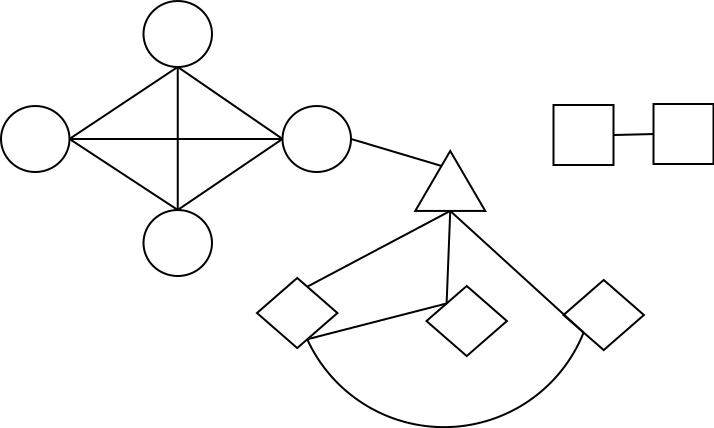
\includegraphics[width=0.7\textwidth]{figures/grafo.png}
\caption{A instância de teste triângulo está ligada ao grafo formado pela classe dos círculos e dos losangos, porém não apresenta ligações com os quadrados.}
\label{fig::grafo}
\end{figure}

Para cada grafo representando uma classe, podemos calcular a credibilidade do exemplo de teste para aquela classe e a incorporar ao classificador Bayesiano. Decidimos modificar a Equação~\ref{eqn::classindependence}, sugerindo seguinte fórmula:

\begin{equation}\label{eqn::nbcredgrafo}
P(X|c_{i}) = \prod^{D}_{k=1}{(P(x_k|c_i)) \cdot (\alpha + Cr_{rel}(X,c_i)) } 
\end{equation}

Como na Equação~\ref{eqn::classindependence}, continuamos calculando o produtório dos atributos que compõem o exemplo $X$, porém calculamos também a credibilidade de $X$ em relação a classe $c_i$. Utilizamos um fator $\alpha$ para evitarmos que a falta de uma aresta entre $X$ e instâncias da classe $i$ possa resultar em uma probabilidade nula de que $X$ seja da classe $i$. Note que poderíamos, sem problema algum, juntar as Equações \ref{eqn::classindependence_conteudo} e \ref{eqn::nbcredgrafo} dando origem a um classificador Bayesiano que leva em conta tanto a credibilidade do conteúdo quanto a dos relacionamentos:

\begin{equation}\label{eqn::nbcredcompleta}
P(X|c_{i}) = \prod^{D}_{k=1}{(P(x_k|c_i) \cdot Cr_{cont}(x_k,c_i)) \cdot (\alpha + Cr_{rel}(X,c_i)) } 
\end{equation}


Pelo fato de modelarmos os relacionamentos existentes entre as entidades por meior de grafos, decidimos por utilizarmos as diversas métricas de redes complexas [cite], a fim de explorarmos as propriedades dos grafos criados. Um exemplo simples de uma dessas métricas é contar o número de vizinhos de um vértice, $viz(v,c_j)$. Essa função retornaria o número de conexões o vértice $v$ tem com seus vizinhos que são da classe $c_j$. Partimos do presuposto que se um vértice for importante para uma determinada classe $j$, $viz(v,c_j)$, será um valor superior para aquela classe. Na Figura~\ref{fig::grafo}, a classe losango seria a de maior credibilidade para classificarmos o triângulo, baseando nessa métrica. Outras várias métricas importantes podem ser listadas e combinada, sendo assim, atribuímos toda a Seção~\ref{subsec::pg_metricas_grafos} para maiores detalhes.  


%%%%%%%%%%%%%%%%%%%%------------------------------------------------------------------------------------------------------------------------------------%%%%%%%%%%%%%%%%%%%%%%%%%%%%%%%%%
%%%%%%%%%%%%%%%%%%%%------------------------------------------------------------------------------------------------------------------------------------%%%%%%%%%%%%%%%%%%%%%%%%%%%%%%%%%
%%%%%%%%%%%%%%%%%%%%------------------------------------------------------------------------------------------------------------------------------------%%%%%%%%%%%%%%%%%%%%%%%%%%%%%%%%%
%%%%%%%%%%%%%%%%%%%%------------------------------------------------------------------------------------------------------------------------------------%%%%%%%%%%%%%%%%%%%%%%%%%%%%%%%%%

\section{Classificador \textit{KNN}.}
\label{subsec::cred_knn}

%No decorrer dessa seção, explicaremos o algoritmo dos K vizinhos mais próximos (do inglês, \textit{K-Nearest Neighbor}, KNN). Da mesma forma que fizemos com o \textit{Naïve Bayes}, dedicamos uma seção, Seção~\ref{subsubsec::knn_cred}, exclusivamente para abordarmos o \textit{KNN} integrado a credibilidade. 

O algoritmo dos $K$ vizinhos mais próximos, \textit{KNN}, é conhecido por ser um método de aprendizagem baseado em analogias, ou seja, comparamos o teste com os exemplos contidos no treinamento a fim de conseguirmos encontrar aqueles com maior semelhança. 
Tipicamente, cada exemplo existente é uma tupla de $D$ dimensões e representa um ponto em um espaço $D$-dimensional. 
Quando um novo exemplo de teste, de classe desconhecida, necessita ser classificado, o algoritmo dos $K$ vizinhos mais próximos procura nesse espaço $D$ dimensional pelos $k$ exemplos do treinamento que estão mais perto do teste. 
Por fim, os $k$ vizinhos mais próximos realizam uma votação para escolherem qual será a classe que o teste pertence.
Na figura~\ref{fig::knn} temos um triângulo que representa nosso exemplo de teste, os quadrados e losangos representando os exemplos de treinamento, pertencentes a classe Quadrado e Losango, respectivamente. As orbitas circulares existentes na figura são epicêntricas e servem apenas para fins didáticos.
Por essa figura, vemos a importância do parâmetro $k$ na decisão da classe que um objeto pertence. Considerando que cada objeto tem o mesmo peso na votação, caso tivéssemos $k=1$, escolheríamos a classe bola para o exemplo de teste, entretanto, se tivéssemos $k=5$, escolheríamos a classe Quadrado. Para valores de $k$ entre 2 e 4, como temos 3 vizinhos a uma mesma distância, temos que considerar algum método de desempate. Em nosso trabalho, ordenamos os vizinhos primeiramente pela distância até o teste e depois por um identificador único, dessa forma, minimizamos problemas relativos a ordem como os exemplos de treinamento são apresentados.

\begin{figure}[ht!]
\centering
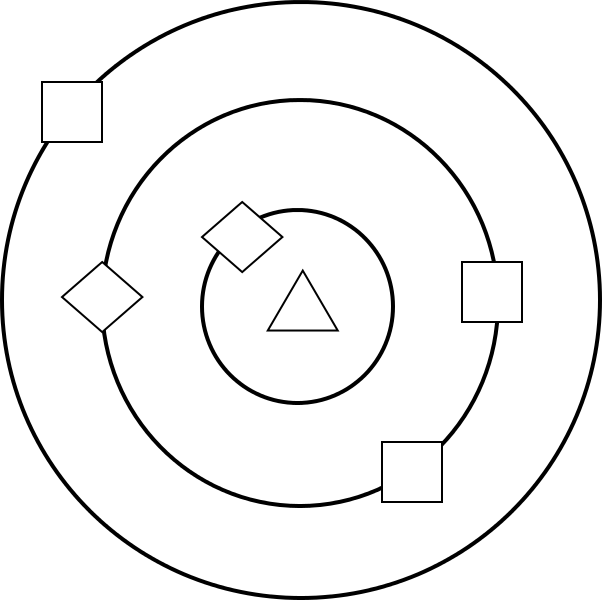
\includegraphics[width=0.5\textwidth]{figures/knn.png}
\caption{O algoritmo dos $k$ vizinhos mais próximos.}
\label{fig::knn}
\end{figure}

Como vimos, uma parte fundamental do \textit{KNN} é podermos calcular o quão próximo uma instância de teste está das instâncias de treinamento. 
Essa proximidade é tipicamente calculada por uma métrica de distância que pode variar de problema para problema. Neste trabalho, utilizamos 3 métricas diferentes, dependendo se estamos classificando um atributo $A_i$ que seja categórico, numérico ou textual. Para duas instâncias $X_1 =  (x_{11}, x_{21}, x_{31}, ..., x_{d1})$ e $X_2 = (x_{12}, x_{22}, x_{32}, ..., x_{d2})$, nas quais $x_{ij}$ representa o valor do atributo $A_i$ para a instância $j$, temos que, caso $A_i$ seja:

\begin{itemize}

\item numérico, utilizamos a distância Euclidiana:

\begin{equation}\label{eqn::distancia_euclidiana}
    dist(X_1, X_2) =  \sqrt{\sum_{i=1}^d (x_{i1}-x_{i2})^2}
\end{equation}

    Com o intuito de evitar que um atributo com grande escala de valores sobreponha um outro atributo de uma menor escala, empregamos a normalização \textit{min-max} para todos os valores $x_i$ do correspondente atributo $A_i$: 

\begin{equation}\label{eqn::distancia_euclidiana}
    x'_{i} =  \frac{x_{i} - min_{A_i}}{ max_{A_i} - min_{A_i} }
\end{equation}

\item categórico, então iremos comparar $X_1$ e $X_2$ e somar uma unidade a distância entre as instâncias para cada $x_i$ que tenha valores distintos entre $X_1$ e $X_2$.

\begin{equation}\label{eqn::distancia_cat}
   dist(X_1, X_2) = \sum_{1 < i < d \ \wedge \ x_{i1} \neq x_{i2}} 1.0
\end{equation}

\item textual, tomamos o a distância dos cosenos entre os dois exemplos $X_1$ e $X_2$ e invertemos o seu sinal. Ou seja, sendo $||X_j|| = \sqrt{x_{1j}^2 + x_{2j}^2 + x_{3j}^2 + ... + x_{dj}^2}$ a norma do vetor representado por um exemplo $X_j$ no espaço e, $x_{ij}$, o peso de um termo $A_i$ no documento $j$, temos que a semelhança entre duas instâncias $X_1$ e $X_2$ pode ser definida como:

\begin{equation}\label{eqn::distancia_texto}
    cosSim(X_1, X_2) = \frac{  x_{i1} \cdot x_{i2} }{ ||X_1|| \cdot ||X_2|| }
\end{equation}

Primeiramente cabe explicar que usamos a métrica \textit{term-frequency - inverse document frequency}, \textit{tf-idf}, como o peso $x_{ij}$ do termo $A_i$ no documento $j$, mais detalhes sobre a métrica \textit{tf-idf} na Seção~\ref{subsubsection::tfidf}. Segundo que, como dito, a métrica acima é chamada de semelhança dos cosenos por se basear no ângulo coseno entre dois vetores no espaço. Como já reparado, estamos interessados na métrica inversa, logo:
 
 \begin{equation}\label{eqn::distancia_texto}
    dist(X_1, X_2) = - cos_sim(X_1, X_2)
\end{equation}


\end{itemize}

\section{Incorporando a credibilidade no \textit{KNN}.}
\label{subsubsec::knn_cred}

De forma paralela ao efetuado nas Seções \ref{subsubsec::nbcredconteudo} e \ref{subsubsec::nbcredgrafos}, iremos em um primeiro momento abordar sobre como incorporar ao \textit{KNN} a credibilidade baseada no conteúdo dos exemplos, Seção \ref{subsubsec::knncredconteudo}. Após isso, na Seção~\ref{subsubsec::knncredgrafos}, analisaremos a credibilidade do ponto de vista das interações entre o exemplo de teste e os exemplos de treinamento, modeladas por meio de grafos.

\subsection{\textit{KNN} com credibilidade baseada no conteúdo.}
\label{subsubsec::knncredconteudo}


Acoplar a credibilidade no algoritmo \textit{Naïve Bayes} é uma tarefa mais imediata do que incorporá-la ao \textit{KNN}, isso se deve a maior homogeneidade do algoritmo Bayesiano. Aqui teremos que trabalhar em cada uma das fórmulas separadamente, sendo que, novamente, buscamos uma maneira de quantificar o relacionamento entre um atributo e uma classe. Note que o \textit{KNN} não realiza essa associação explicitamente, ou seja, como vimos na Seção~\ref{subsec::cred_knn}, somente observamos a classe pertencente a uma instância de treinamento quando já temos os $k$ vizinhos mais próximos definidos e estamos votando para saber qual a classe a ser escolhida.

O \textit{KNN} é um algoritmo que, de uma maneira geral, compara duas instâncias, uma do conjunto de treinamento e outra do teste, e baseia-se em algum cálculo respectivo a um mesmo atributo $A_i$ de cada uma das instâncias. O que tentamos fazer é utilizar o conhecimento de qual classe a instância de teste pertence e avaliarmos o quanto de credibilidade o valor $x_i$ de um determinado atributo $A_i$ nos provê em relação aquela classe $c_j$ da instância de treino.

Efetivamente em nossos testes, empregamos a credibilidade para classificação textual e categórica. Embora acreditamos que seja perfeitamente possível utilizarmos o mesmo raciocínio para definirmos a credibilidade em atributos numéricos, deixamos essa tarefa como trabalho futuro. A seguir, nas Seções~\ref{subsubsec::knncat} e~\ref{subsubsec::knntexto}, apresentamos as modificações realizadas no algoritmo dos $k$ vizinhos mais próximos para os atributos categóricos e textuais, respectivamente.

\subsubsection{\textit{KNN} categórico.}
\label{subsubsec::knncat}

Procuramos, ao desenvolver as modificações seguintes, ter em vista dois fatos importantes:
\begin{enumerate}
\item se a instância de treinamento e a de teste têm os mesmos valores para todos os seus atributos, então a distância entre as mesmas é zero. 
\item uma instância de treino que apresenta diferença em $T$ atributos da instância de teste, tende a ter uma distância menor que outra que apresente $T+1$ atributos distintos.
\end{enumerate}

A regra 1 é bastante simples, não criamos uma distância de onde a mesma não existe. A regra 2 diz que ao levar em consideração a classe da instância de treinamento, iremos criar uma pertubação no espaço, porém queremos que essa pertubação seja controlada de forma a continuarmos podendo recorrer à hipótese básica do \textit{KNN} de que instâncias parecidas, ou seja, com grande número de atributos iguais, estão bem próximas em uma distribuição espacial.

Visualmente, o que queremos com a modificação realizada no algoritmo dos vizinhos mais próximos, está expresso na Figura~\ref{fig::KNNantesedepois}. Em~\ref{fig::KNNantesedepois}-(a) temos a situação já discutida anteriormente, composta de um exemplo do treino que difere em uma característica, três que diferem em duas e um outro que difere em três, sendo que esses são os cinco vizinhos mais próximos de nosso exemplo de teste. Por sua vez, na Figura~\ref{fig::KNNantesedepois}-(b) temos os mesmos exemplos mostrados, porém com as distâncias entre o teste e o treino sendo comparadas utilizando o conhecimento sobre a qual classe pertence o exemplo de treino. Pode-se observar que as instâncias da classe Quadrado foram mais afetadas, podendo significar que o exemplo de teste pertença a classe Losango. Dessa vez, ao contrario do que teríamos na situação anterior, para valores de $k$ entre 1 e 3, sabemos definir que o teste pertence a classe dos losangos, sem precisarmos utilizar uma métrica especial de desempate. 

\begin{figure}[ht]
\centering
\subfloat[\textit{KNN} original]{
    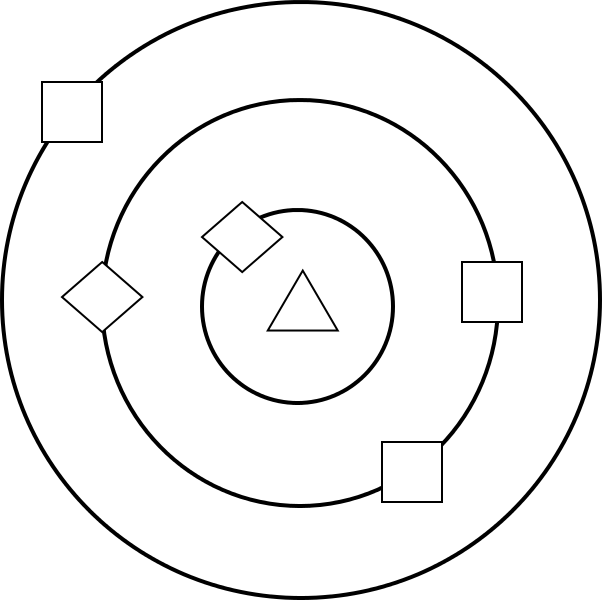
\includegraphics[width=0.5\textwidth]{figures/knn.png}
}
\subfloat[\textit{KNN} com credibilidade]{
    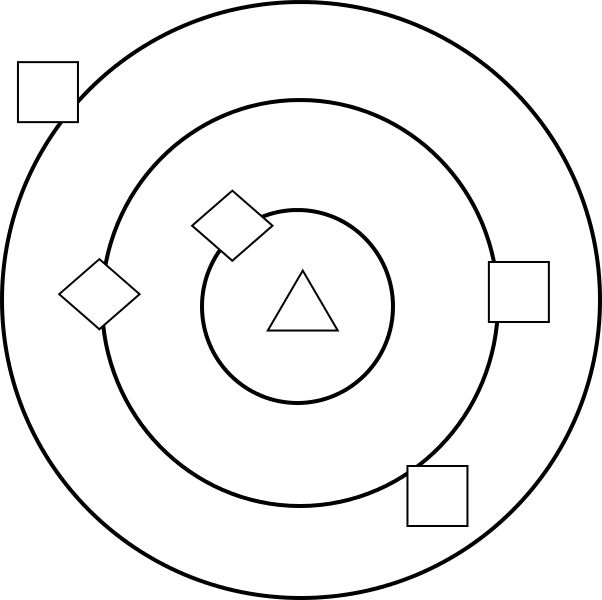
\includegraphics[width=0.5\textwidth]{figures/knncred.png}
}
\caption{Em (a) temos o algoritmo original dos $K$ vizinhos mais próximos e em (b) temos um possível resultado da utilização da credibilidade conjuntamente ao \textit{KNN}.  
\label{fig::KNNantesedepois}}
\end{figure}

Levando em consideração o que foi mostrado até esse ponto, sendo $X_1$ a instância de teste, $X_2$ a de treino e $c_{X_2}$ a classe a qual nossa instância de treinamento pertence, modificamos a Equação~\ref{eqn::distancia_cat} para:

\begin{equation} \label{eqn::distancia_cat_cred}
   dist(X_1, X_2) = \sum_{1 < i < d \ \wedge \ x_{i1} \neq x_{i2}} 1.0 + \frac{1.0}{1.0 + Cr_{cont}(x_{i1}, c_{X_2} ))}
\end{equation}

Para estarmos de acordo com o efeito mostrado na Figura \ref{fig::KNNantesedepois}, apenas adicionamos um termo relacionado a credibilidade na Equação~\ref{eqn::distancia_cat}, um fator inversamente proporcional ao valor calculado para a credibilidade. Note que teríamos os mesmos resultados se excluíssemos o primeiro 1.0 existente dentro do somatório da equação acima, porém o que faríamos seria aproximar os exemplos com maior credibilidade ao invés de afastar os com menor.

\subsubsection{\textit{KNN} textual.}
\label{subsubsec::knntexto}

Decidimos, assim como feito na incorporação da credibilidade nos atributos categóricos, apenas utilizar a credibilidade relacionada ao termo do teste e a classe do exemplo de treinamento. Dessa forma, modificamos a Equação \ref{eqn::distancia_texto}, resultando em:

\begin{equation}\label{eqn::distancia_texto_cat}
    dist(X_1, X_2) = \frac{  Cr_{cont}(x_{i1}, c_{X_2}) \cdot x_{i1} \cdot x_{i2} }{ ||X'_1|| \cdot ||X_2|| }
\end{equation}

Repare que utilizamos $||X'_1||$ como a norma do vetor $X_1$, levando em conta a credibilidade em relação à classe da instância de treino $X_2$, logo teríamos que $||X'_1|| = \sqrt{ ( Cr_{cont}(x_{11}, c_{X_2}) \cdot x_{11} )^2 + ( Cr_{cont}(x_{21}, c_{X_2}) \cdot x_{21} )^2 +  ... +  ( Cr_{cont}(x_{d1}, c_{X_2}) \cdot  x_{d1} )^2}$.
Novamente, assim como discutido na Seção~\ref{subsubsec::nbcredconteudo}, existem diversas métricas que podemos utilizar para inferirmos a credibilidade de um elemento, a fim de melhorarmos a capacidade do algoritmo \textit{KNN} em classificar. Algumas dessas métricas já foram previamente discutidas e o serão novamente ao longo desse trabalho, entretanto, voltamos a frisar que a escolha de uma função de credibilidade é dependente ao contexto que a mesma está inserida e combinar as métricas disponíveis é uma tarefa combinacional cara e, para tanto, estamos usando Programação Genética como será discutido em detalhes no Capítulo~\ref{cap::programacao_genetica}.

\subsection{\textit{KNN} com credibilidade baseada em relacionamentos.}
\label{subsubsec::knncredgrafos}

Exatamente a mesma situação exposta com detalhes na Seção~\ref{subsubsec::nbcredgrafos} retoma à cena. Ou seja, modelamos a credibilidade atribuída a uma instância de teste em relação a determinada classe utilizando o relacionamento que aquela instância tem com as demais instâncias de treino, levando em consideração a classe que as mesmas pertencem. Diferentemente da modelagem da credibilidade para o conteúdo do algoritmo \textit{KNN}, dessa vez, podemos criar apenas um modelo que se adapta a qualquer tipo de atributo, numérico, categórico ou textual. Logo, sendo $X_1$ a instância de teste, $X_2$ a instância de treino e $\alpha$ o fator somado a credibilidade de relacionamento para evitarmos valores nulos no denominador, temos:

\begin{equation}\label{eqn::distancia_grafos}
%    dist(X_1, X_2) = dist(X_1, X_2) \cdot (\alpha + Cr_{rel}(X_1, class_{X_2})) 
    dist(X_1, X_2) = \frac{ dist(X_1, X_2) } { \alpha + Cr_{rel}(X_1, class_{X_2}) }
\end{equation}

Note que estamos modificando o valor da distância calculado entre a instância de teste e a de treino, baseando no fato que quanto maior a credibilidade do relacionamento do teste $X_1$ a uma classe $c_i$, menor será a distância entre o exemplo $X_1$ e os outros exemplos do treinamento que pertencem a classe $c_i$.

Mais uma vez, podemos utilizar as várias propriedades dos grafos para calcularmos a credibilidade dos relacionamentos. Na Seção~\ref{subsec::pg_metricas_grafos} temos definidas várias métricas que calculam essas propriedades. Por fim, usamos a Programação Genética para combinarmos essas métricas a fim de obtermos uma melhor função de credibilidade que explore o melhor possível o relacionamento exemplo-classe.

